\section{Operationelle Semantik \small (Vorlesung 2 am 24.04.)}
\subsection{Operationelle Semantik am Beispiel der Terme}
\marginnote{\small\emph{(Inhalt ist nicht im Lehrbuch!)}}[0cm]
%notes:
% auf höhe interpreter gfx!
\marginnote{\small \textbf{AST:} abstract syntax tree}[8,5cm]
Es ist wichtig die Struktur von einer Sprache zu kennen, erst dann kann man eine korrekte Interpretation anfertigen!\\
Grundsätzlich gibt es zwei Methoden:
\begin{compactitem}
	\item[\textbf{Übersetzer}] Zu jedem Programm ein äquivalentes Maschinenprogramm erstellen.\\
\begin{tikzpicture}[node distance = 4cm, auto]
    % Place nodes
    \node [block] (comp) {Übersetzer (Syntaxanalyse)};
    \node [cloud, left of=comp] (prog) {Programm};
    \node [cloud, right of=comp, align=center] (mprog) {Maschinen-\\programm};
    \node [block, below of=mprog, node distance=3cm] (abstractmachine) {abstrakte Maschine};
    \node [cloud, left of=abstractmachine] (ausg) {Ausgabe};
    \node [cloud, right of=abstractmachine] (eing) {Eingabe};
    % Draw edges
    \path [line] (prog) -- (comp);
    \path [line] (comp) -- (mprog);
    \path [line] (mprog) -- (abstractmachine);
    \path [line] (abstractmachine) -- (ausg);
    \path [line] (eing) -- (abstractmachine);
\end{tikzpicture}	
	\item[\textbf{Interpreter}] Das Programm wird mit Eingabe zum Maschinenprogramm transferiert.\\
\begin{tikzpicture}[node distance = 4cm, auto]
    % Place nodes
    \node [block] (syn) {Syntaxanalyse};
    \node [cloud, left of=syn, align=center] (prog) {Programm\\+\\Eingabe};
    \node [block, right of=syn, node distance=5cm] (abstractmachine) {abstrakte Maschine};
    \node [cloud, right of=abstractmachine] (ausg) {Ausgabe};
    % Draw edges
    \path [line] (prog) -- (syn);
    \path [line] ([yshift=3em]syn) -- node {AST}([yshift=3em]abstractmachine);
    \path [line] ([yshift=-3em]syn) -- node [below] {Eingabe}([yshift=-3em]abstractmachine);
    \path [line] (abstractmachine) -- (ausg);
\end{tikzpicture}
\end{compactitem}
\subsection{Terme der Sprache WHILE}
\begin{lstlisting}[mathescape]
// Terme TERM
T::= Z  |  I  |  T$_1$ OP T$_2$ | READ, für T$_1$,T$_2$ in TERM
\end{lstlisting}

\subsubsection*{Beispiel: AST}
Der Ausdruck
\begin{lstlisting}
3 + read - x 
\end{lstlisting}
wird zu:\\
\begin{tikzpicture}[-,>=stealth',level/.style={sibling distance = 5cm/#1, level distance = 1.5cm}] 
\node [node]{-}
	child{node [node]{+}
		child{ node [node]{3}}
		child{ node [node]{read}}
	}
	child{node [node]{x}};
\end{tikzpicture}

\subsection{Informelle Semantik}
Interpretation nur möglich, wenn Speicher und Eingabe vorgelegt sind.\\
\textbf{Annahme:} wir bekommen alles als AST und wir bekommen eine Eingabe, die auch von der Maschine unterstützt wird!
\begin{compactitem}
	\item[\textbf{Übersetzer}] 
		\textbf{Idee:} depth-first-left-to-right-postorder Traversierung des AST
		Unser Beispiel:\\
		\begin{tikzpicture}[-,>=stealth',level/.style={sibling distance = 5cm/#1, level distance = 1.5cm}] 
		\node [node]{-}
			child{node [node]{+}
				child{ node [node]{3}}
				child{ node [node]{read}}
			}
			child{node [node]{x}};
		\end{tikzpicture}
		wird übersetzt zu:\\
	\begin{lstlisting}
PUSH 3
READ
ADD
LOAD x
SUB
		\end{lstlisting}
		Zustandsveränderungen:\\
		aktueller Zustand (siehe Bild Architektur!):
\begin{align*}
<\epsilon|S|8.5. ...> &\xrightarrow{\text{\lstinline!PUSH 3!}} &<3.|S|8.5. ...> \\
&\xrightarrow{\text{\lstinline!READ!}} &<-8.3-\epsilon|S|5. ...> \\
&\xrightarrow{\text{\lstinline!ADD!}} &<3+(-8).\epsilon|S|5. ...> \\
&\xrightarrow{\text{\lstinline!LOAD x!}} &<2.-5.\epsilon|S| ...5> \\
&\xrightarrow{\text{\lstinline!SUB!}} &<-7.\epsilon|S|5...>
\end{align*}
Semantik eines Terms $T$ zu geg. Speicher $S$ und Eingabe $E$ ist die Spitze des Wertekellers(STACK) nach Ausführung von trans $T$ auf $<\epsilon|S|E>$, falls diese Ausführung fehlerfrei läuft, sonst Fehler!\\
	\item[\textbf{Interpreter}] (abstrakte Maschine beinhaltet eine Komponente (Kontrollkeller), in der ASTs in einem Keller gespeichert werden können.)
	\begin{compactitem}
		\item Kontrollkeller
		\item Zustand der abstrakten Maschine hat Komponenten
			\begin{compactitem}
				\item Wertekeller $W$ ($\in ZAHL^*$)
				\item Speicher $S$ ($S \in [ID \rightarrow ZAHL]$)
				\item Kontrollkeller $K$ ($ \in (AST \cup OP)^*$)
				\item Eingabe $E$ ($\in ZAHL^*$)
			\end{compactitem}
	\end{compactitem}
		Zur Formalisierung der Semantik über die abstrakte Maschine mit dem Zustandsraum Z durch Angabe von:
		\begin{compactitem}
			\item[\textbf{(i)}] einem Anfangszustand $Z_{T,S,E}$ für jeden Term $T$, Speicher $S$ und Eingabe $E$.
			\item[\textbf{(ii)}] eine Zustandsüberführungsfunktion $\Delta : Z \rightarrow Z$ (partiell)
			\item[\textbf{(iii)}] Erklärung der Semantik über Iteration von $\Delta$\\		
		\end{compactitem}
		für Terme aus WHILE:
			\begin{compactitem}
				\item[\textbf{(i)}]	$Z_{T_0,S_0,E_0} := <\epsilon|S_0|T_0.\epsilon|E_0>$
				\item[\textbf{(ii)}] $\Delta$ per Induktion über die Struktur der Kontrollkellerspitze\\
					\begin{align*}
						&\Delta <W|S|n.K|E> &= &<n.W|S|K|E> \text{für alle } n \in ZAHL, W,S,E \text{ wie oben.}\\
						&\Delta <W|S|x.K|E> &= &<s(x).W|S|K|E> \text{für alle } x \in ID\\
						&\Delta <W|S|read.K|n.E> &= &<n.W|S|K|E> \text{für alle } n \in ZAHL\\
						&\Delta <W|S|T_1 OP T_2.K|E> &= &<W|S|T_1.T_2.OP.K|E> \\
						&\Delta <n_2.n_1.W|S|OP.K|E> &= &<n_1 OP n_2.W|S|K|E> n_1, n_2 \in ZAHL \text{ falls } n_1 OP n_2 \text{ definiert ist.}\\
					\end{align*}
				\item[\textbf{(iii)}] Die Semantik eines (beliebigen) Terms $T$ im Bezug auf einem Speicher $S$ und eine Eingabe $E$ ist $n \in ZAHL$, wenn $\Delta^k Z_{T,S,E} = <n.\epsilon|S|\epsilon|E'>$ für beliebige $E' \in ZAHL^*$, undefiniert sonst!\\ 		
			\end{compactitem}		
\end{compactitem}

\subsubsection*{Architektur der abst. Maschine}
\begin{figure}[h]
	\centering
	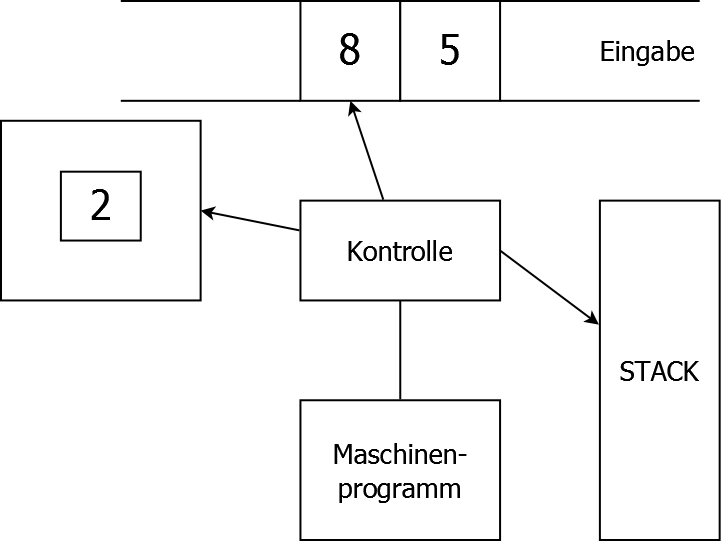
\includegraphics[width=300px]{../gfx/architecture.png}
\end{figure}

\subsubsection*{Befehlssatz}
\begin{lstlisting}
// Stack und Speicher Operationen
READ 				// lese Zahl v. Eingabe, PUSH Zahl, rücke Zeiger um eins weiter
LOAD x			// PUSH Inhalt aus Speicher mit symbl. Adr. x
PUSH n			// für jede Zahl aus N lege n auf Stack
(STORE x) 	// belegt Speicher mit der symbolischer Adresse x 
(GOTO n) 		// bedingter Sprung

// arithmetische Operationen
ADD
MULT
SUB
\end{lstlisting}




